\clearpage\begingroup\SourceLeaf{114b}\HistoricalHead{109}{R}{GAUSS AN OLBERS UND SCHUMACHER.}
\newcommand{\HistoricalCurrencyTwentyThreeA}{%
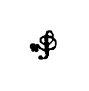
\begin{tikzpicture}[x=0.1666667pt,y=-0.1666667pt,baseline=-11pt]
\path[use as bounding box] (0,0) rectangle (71,77);
\path[fill=black,even odd rule] (51,6) -- (44,6) -- (43,7) -- (42,7) -- (40,9) -- (40,11) -- (39,12) -- (39,14) -- (36,17) -- (35,17) -- (34,18) -- (32,18) -- (29,21) -- (28,21) -- (26,23) -- (26,31) -- (29,34) -- (30,34) -- (32,36) -- (33,36) -- (36,38) -- (36,40) -- (37,41) -- (37,45) -- (36,46) -- (30,44) -- (26,40) -- (26,39) -- (22,35) -- (20,35) -- (17,37) -- (14,34) -- (9,34) -- (8,35) -- (7,35) -- (5,38) -- (5,44) -- (8,47) -- (8,50) -- (10,52) -- (13,52) -- (14,51) -- (15,51) -- (18,53) -- (20,53) -- (24,49) -- (24,48) -- (22,46) -- (23,45) -- (24,45) -- (26,47) -- (29,47) -- (34,51) -- (36,51) -- (37,52) -- (37,53) -- (38,54) -- (38,56) -- (39,57) -- (39,60) -- (35,65) -- (34,65) -- (31,62) -- (31,61) -- (30,60) -- (26,60) -- (23,63) -- (23,67) -- (26,69) -- (32,69) -- (33,68) -- (40,68) -- (41,67) -- (42,67) -- (44,65) -- (44,63) -- (46,60) -- (46,51) -- (49,48) -- (56,48) -- (57,47) -- (58,47) -- (58,46) -- (61,43) -- (61,41) -- (62,40) -- (62,38) -- (63,37) -- (63,31) -- (62,30) -- (62,27) -- (56,21) -- (56,17) -- (57,16) -- (56,15) -- (56,14) -- (55,13) -- (55,12) -- (54,11) -- (53,8) -- cycle
(57,28) -- (59,31) -- (59,39) -- (57,41) -- (54,42) -- (52,44) -- (50,44) -- (49,45) -- (47,45) -- (45,43) -- (47,37) -- (48,36) -- (49,36) -- (49,35) -- (50,34) -- (51,34) -- (52,33) -- (52,32) -- (56,28) -- cycle
(46,22) -- (47,23) -- (51,23) -- (53,25) -- (53,27) -- (47,33) -- (45,31) -- (45,30) -- (44,29) -- (45,28) -- (45,23) -- cycle
(34,22) -- (35,22) -- (36,23) -- (36,28) -- (37,29) -- (37,31) -- (35,33) -- (34,33) -- (30,29) -- (30,25) -- (32,23) -- (33,23) -- cycle
(44,13) -- (47,10) -- (48,10) -- (52,14) -- (53,17) -- (52,18) -- (50,18) -- (49,17) -- (46,17) -- (44,15) -- cycle;
\end{tikzpicture}}
\newcommand{\HistoricalCurrencyTwentyThreeB}{%
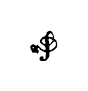
\begin{tikzpicture}[x=0.1666667pt,y=-0.1666667pt,baseline=-11pt]
\path[use as bounding box] (0,0) rectangle (70,76);
\path[fill=black,even odd rule] (50,7) -- (46,7) -- (45,8) -- (44,8) -- (41,11) -- (41,13) -- (40,14) -- (40,16) -- (37,19) -- (36,19) -- (35,20) -- (33,20) -- (28,25) -- (28,26) -- (27,27) -- (27,32) -- (31,36) -- (32,36) -- (34,38) -- (35,38) -- (38,41) -- (38,42) -- (39,43) -- (39,47) -- (38,48) -- (33,48) -- (31,46) -- (30,46) -- (21,37) -- (19,39) -- (17,39) -- (15,37) -- (14,37) -- (13,36) -- (10,36) -- (6,40) -- (6,45) -- (7,46) -- (7,48) -- (9,50) -- (9,53) -- (10,53) -- (11,54) -- (19,54) -- (21,56) -- (22,56) -- (24,53) -- (24,50) -- (22,48) -- (21,45) -- (22,44) -- (24,44) -- (26,46) -- (26,47) -- (27,48) -- (30,49) -- (32,51) -- (34,51) -- (36,53) -- (38,53) -- (40,55) -- (40,58) -- (39,59) -- (39,66) -- (36,69) -- (34,67) -- (34,63) -- (33,62) -- (29,62) -- (26,65) -- (26,70) -- (29,72) -- (38,72) -- (39,71) -- (40,71) -- (43,68) -- (43,67) -- (46,64) -- (46,63) -- (47,62) -- (47,54) -- (49,52) -- (50,52) -- (51,51) -- (53,51) -- (55,49) -- (57,49) -- (63,43) -- (63,42) -- (64,41) -- (64,33) -- (63,32) -- (63,30) -- (62,29) -- (62,28) -- (57,23) -- (57,19) -- (56,18) -- (56,15) -- (54,13) -- (54,11) -- cycle
(10,43) -- (11,42) -- (13,42) -- (14,43) -- (14,44) -- (13,45) -- (11,45) -- (10,44) -- cycle
(59,30) -- (61,32) -- (61,39) -- (60,40) -- (60,41) -- (56,45) -- (55,45) -- (52,48) -- (49,49) -- (46,46) -- (47,45) -- (47,39) -- (48,38) -- (50,38) -- (50,37) -- (55,32) -- (55,31) -- (56,30) -- cycle
(33,25) -- (37,25) -- (38,26) -- (38,31) -- (39,32) -- (39,34) -- (38,35) -- (35,35) -- (34,34) -- (33,34) -- (32,33) -- (32,31) -- (31,31) -- (30,30) -- (30,29) -- (32,27) -- (32,26) -- cycle
(47,23) -- (48,23) -- (49,24) -- (52,25) -- (54,27) -- (54,29) -- (51,32) -- (51,33) -- (49,35) -- (47,35) -- (46,34) -- (46,29) -- (45,28) -- (45,26) -- cycle
(45,16) -- (49,12) -- (50,12) -- (54,16) -- (54,18) -- (55,19) -- (55,20) -- (54,21) -- (51,21) -- (50,20) -- (46,20) -- (45,19) -- cycle;
\end{tikzpicture}}
\newcommand{\HistoricalCurrencyTwentySix}{%

\begin{tikzpicture}[x=0.1250000pt,y=-0.1250000pt,baseline=-11pt]
\path[use as bounding box] (0,0) rectangle (90,99);
\path[fill=black,even odd rule] (67,10) -- (64,10) -- (63,9) -- (56,9) -- (55,10) -- (55,11) -- (54,12) -- (52,12) -- (51,13) -- (51,15) -- (50,16) -- (49,16) -- (49,21) -- (47,23) -- (44,23) -- (42,25) -- (39,25) -- (38,26) -- (36,26) -- (35,29) -- (33,31) -- (33,40) -- (39,46) -- (39,48) -- (41,50) -- (44,50) -- (48,55) -- (48,59) -- (45,62) -- (42,62) -- (41,61) -- (40,61) -- (31,52) -- (31,51) -- (30,50) -- (30,48) -- (27,45) -- (25,45) -- (21,49) -- (19,49) -- (15,45) -- (9,45) -- (5,49) -- (5,55) -- (3,57) -- (3,58) -- (5,60) -- (7,60) -- (9,62) -- (9,65) -- (12,68) -- (19,68) -- (21,70) -- (25,70) -- (28,67) -- (28,64) -- (27,63) -- (27,62) -- (26,62) -- (25,61) -- (25,60) -- (28,57) -- (31,60) -- (33,60) -- (34,61) -- (35,61) -- (38,64) -- (40,64) -- (42,66) -- (42,67) -- (45,67) -- (46,68) -- (48,68) -- (49,69) -- (49,83) -- (48,84) -- (48,85) -- (45,88) -- (44,88) -- (41,85) -- (43,83) -- (38,79) -- (34,79) -- (32,81) -- (29,82) -- (29,85) -- (31,87) -- (31,89) -- (33,91) -- (36,91) -- (39,94) -- (43,94) -- (44,93) -- (48,93) -- (50,91) -- (51,91) -- (55,87) -- (55,86) -- (58,83) -- (58,70) -- (63,65) -- (64,65) -- (65,64) -- (67,64) -- (68,63) -- (71,63) -- (73,61) -- (74,61) -- (80,55) -- (80,52) -- (81,51) -- (81,50) -- (83,48) -- (83,39) -- (81,37) -- (81,36) -- (73,28) -- (73,26) -- (74,25) -- (74,20) -- (71,17) -- (71,16) -- (70,15) -- (70,13) -- (69,12) -- (68,12) -- (67,11) -- cycle
(75,39) -- (78,42) -- (78,47) -- (77,48) -- (77,50) -- (75,52) -- (75,54) -- (71,58) -- (68,58) -- (65,61) -- (62,61) -- (61,62) -- (59,62) -- (57,60) -- (57,58) -- (58,57) -- (58,51) -- (61,48) -- (66,48) -- (67,47) -- (67,46) -- (69,44) -- (70,44) -- (70,42) -- (73,39) -- cycle
(42,32) -- (44,32) -- (45,33) -- (45,34) -- (48,36) -- (48,42) -- (45,45) -- (41,41) -- (41,39) -- (40,38) -- (40,35) -- cycle
(61,29) -- (65,29) -- (68,32) -- (68,36) -- (67,37) -- (67,39) -- (63,43) -- (61,43) -- (58,40) -- (58,32) -- (59,31) -- (60,31) -- (60,30) -- cycle
(61,15) -- (64,15) -- (68,19) -- (68,21) -- (69,22) -- (69,24) -- (67,26) -- (65,26) -- (64,25) -- (61,25) -- (60,24) -- (60,23) -- (58,23) -- (57,22) -- (57,19) -- cycle;
\end{tikzpicture}}

\begin{center}[23.]\end{center}
\begin{center}\textsc{Gauss} an \textsc{Schumacher}.\quad Göttingen, 24. Juni 1836.\end{center}
\begin{center}\begin{minipage}{.82\linewidth}\centering\hrule\vspace{3pt}
\small [Briefwechsel zwischen \textsc{Gauss} und \textsc{Schumacher} III, S. 73.]
\par\vspace{3pt}\hrule\end{minipage}\end{center}
\noindent .\ .\ .\ .\ .\ .\ .\ .\ .\ .\ .\ .\ .\ .\ .\ .\ .\ .\ .\ .\ .\par
\indent \textsc{Steinheil} führt jetzt (als Probeversuch für künftig weiter zu erstreckende
magnetische Telegraphie) eine Drahtleitung von München nach Bogenhausen,
bei welcher Gelegenheit er schon eine interessante Bemerkung gemacht hat —
meinem Vermuthen nach in der atmosphärischen Electricität begründet, welche
sich also an den Magnetometern ausserordentlich stark sichtbar machen lässt.
\clearpage\SourceLeaf{115}\HistoricalHead{110}{L}{PHYSIK. BRIEFWECHSEL.}
\indent Für die magnetische Telegraphie zwischen Leipzig und Dresden sind dem
Vernehmen nach 8000 \HistoricalCurrencyTwentyThreeA\ ausgesetzt, namentlich zuerst 2000 \HistoricalCurrencyTwentyThreeB\ für die Bahnstrecke
von Leipzig nach Wurzen. Ich höre dies von \textsc{Weber}, bin aber ungewiss,
ob die Notiz schon bekannt werden darf.
\begin{flushright}Stets der Ihrige\hspace*{.18\linewidth}\\[6pt]
C. F. G.\hspace*{.12\linewidth}\end{flushright}
\clearpage\endgroup
